\chapter{Simulation of $pp$ Collision Events}
\label{chap:simulation}


%from: http://imaginaryinstruments.org/lovelace-analytical-engine/
\epigraph{\textit{[The Analytical Engine] might act upon other things besides number, were objects found whose
fundamental relations could be expressed by those of the abstract science of operations, and which should be also susceptible
of adaptations to the action of the operating notation and mechanism of the engine. Supposing, for instance, that the
fundamental relations of pitched sounds in the science of harmony and of musical composition were susceptible of such
expression and adaptations, the engine might compose elaborate and scientific pieces of music of any degree of
complexity or extent.}}{--Ada Augusta, Countess of Lovelace}

In order to be able to make predictions with which comparisons to the observed data
recorded by the ATLAS data can be made, the need for an accurate simulation infrastructure
arises.
Simulation of the $pp$ collision process must be made in order to estimate predicted
rates of specific SM processes so that, in searches for new physics, one can
construct a reliable \textit{background-only} model with which the compatibility of data
and the \textit{background-plus-signal} model, in which a BSM physics process is additionally simulated,
can be tested {\color{red}{NEEDS RE-WORDING}}.
In addition to computing overall rates and kinematics of specific physics processes, an accurate
simulation of the response of the ATLAS detector to these physics events must also be performed which
requires accurate knowledge of the detector material as well as its read-out such that these, too,
may be simulated.

%Physics analyses at ATLAS generally rely on simulations of $pp$ collisions,
%and of particular procecesses such as the production of $W$ bosons, in order to build
%a model of how the known SM processes behave.
%By 

\section{QCD Factorization and Fragmentation}
\label{sec:fact_frag}

\begin{figure}[!htb]
    \begin{center}
        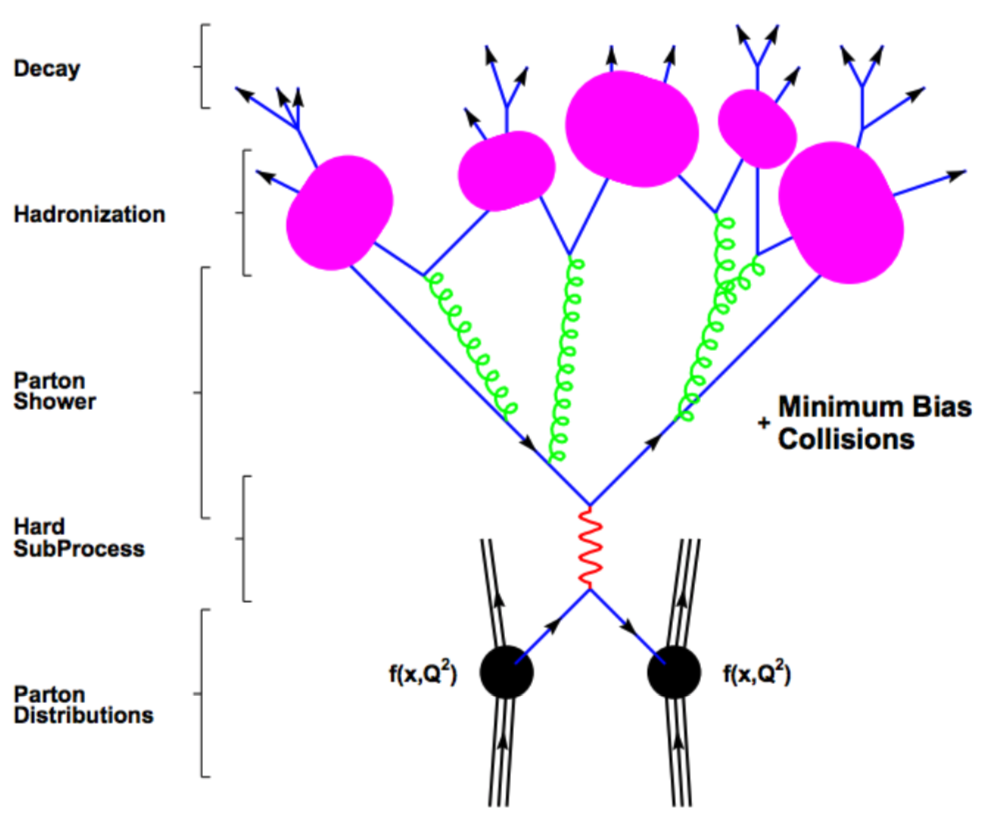
\includegraphics[width=0.6\textwidth]{figures/event_simulation/pp_simulation_steps}
        \caption{
            Cartoon illustrating the concepts of QCD factorisation and fragmentation as regards
            the $pp$ interactions at the LHC.
            {\color{red}{redo this figure}}
        }
        \label{fig:pp_sim_steps}
    \end{center}
\end{figure}

Before simulation of the ATLAS detector response can take place, accurate calculation and simulation of the production of final
state particles as a result of a $pp$ collision must occur.
The steps of such simulation are illustrated in Figure~\ref{fig:pp_sim_steps}.
The breakdown of steps illustrated in Figure~\ref{fig:pp_sim_steps} represent the main characterising features
of QCD, namely: 
\begin{itemize}
    \item Asymptotic freedom (confinement)
    \item Renormalisation group equations (running of scales / scale dependence)
    \item Factorisation (separation of high- and low-energy (perturbative and non-perturbative) regimes)
\end{itemize}

The asymptotic freedom and confinement of QCD state that the strength of the strong coupling, $\alpha_s$, becomes weak at
small distances (high energy scales, $Q^2$) and strong at a large distance.
It is asymptotic freedom that enables the use of perturbative QCD (pQCD) to calculate the hard-scatter (large $Q^2$)
reactions in QCD. Additionally, asymptotic freedom makes the color force dependent on the choice of scale, $Q^2$,
making it necessary to perform computations with respect to a reference scale.
This forces the introduction of arbitrary scales, $\mu$, that are the reference scales enabling the pQCD computations
to proceed but on which physical observables should not depend.
This last requirement leads to the renormalisation group equations that relate pQCD expressions at a given
scale, $\mu$, to physical observables.

The factorisation implied by the above allows us to separate hard-scatter processes from the soft (low energy) parts
of QCD that cannot be calculated perturbatively.
These nonperturbative regimes occur at the characteristic scales of confinment onset, at $Q \sim \Lambda$ ($\sim 200\,\MeV$).
At scales above $m_{\text{hadron}} \sim 1\,\GeV$, the perturbative treatment becomes viable.
%In $pp$ collisions, the parton distribution functions (PDFs) absorb the non-perturbative aspects of the process
%computation and parameterise the probability to find a given parton in the proton holding some fraction of its momentum.
%Being incalculable, the PDFs must be measured in data in separate experiments and are taken
%as input to pQCD calculation, providing the initial conditions of the participating partons at some scale $\mu$ {\color{red}{to which it is evolved using DGLAP}}.
%The remaining computation of the hard-scatter of the initial partons can then be performed using the machinery
%of pQCD.
\begin{align}
    \sigma_{pp \rightarrow X} = \sum\limits_{A,B} \int\limits_0^1 \mathrm{d}x_A \int\limits_0^1 \mathrm{d}x_B \: f_{A}(x_A, \mu_F^2) \, f_{B}(x_B, \mu_F^2) \times \hat{\sigma}_{AB \rightarrow X}(x_A p_A, x_B p_B, \mu_F^2, \mu_R^2)
    \label{eq:pp_xsec}
\end{align}
This factorisation of QCD implies that calculations of $pp$ collision processes take the form of Equation~\ref{eq:pp_xsec},
where the sum runs over the partons of types $A$ and $B$ that exist in the incident protons and that contribute to the hard-scatter process.
The PDFs, $f_{i}(x_i, \mu_F^2)$, absorb the non-perturbabitve aspects of the computation and parameterise the probability
to find a given parton in the proton carrying a fraction of the proton's momentum, $x_i$, evaluated at a given energy scale
$Q^2 = \mu_F^2$.
As the PDFs describe the non-perturbative initial conditions of the partons initiating the hard-scatter processes,
they are incalculable and must be obtained from subsidiary measurements or from altogether
different experiments that are dedicated to their measurement~\cite{Placakyte:2011az,Ball:2012cx}.
The PDFs are measured at specific scales $Q^2$ and are then extrapolated to the energy regime relevant to the physics process
being calculated.
This extrapolation is governed by the Dokshitser-Gribov-Lipatov-Altarelli-Parisi (DGLAP)
evolution equations which evolve the PDFs from one scale to another~\cite{Altarelli:1977zs,Gribov:1972ri,Dokshitzer:1977sg}.
The parton-level cross-section, $\hat{\sigma}_{AB \rightarrow X}$, describes the hard-scatter between the initiating partons
and can be calculated using the machinery of perturbation theory.
Both the PDFs and parton-level cross-section are dependent on the \textit{factorisation scale}, $\mu_F$,
which defines the cut-off scale below which phenomena are absorbed in the PDFs and above which phenomena contribute to the
hard-scatter. 
As with all calculations involving the perturbation theory of QFT, the parton-level cross-section also depends on the
renormalisation scale, $\mu_R$, defining the ultra-violet cut-off scale.
Examples of proton PDFs, measured using data inclusive of $14\,\TeV$ data from the LHC, are provided in Figure~\ref{fig:pdfs_lhc}.

\begin{figure}
    \begin{center}
        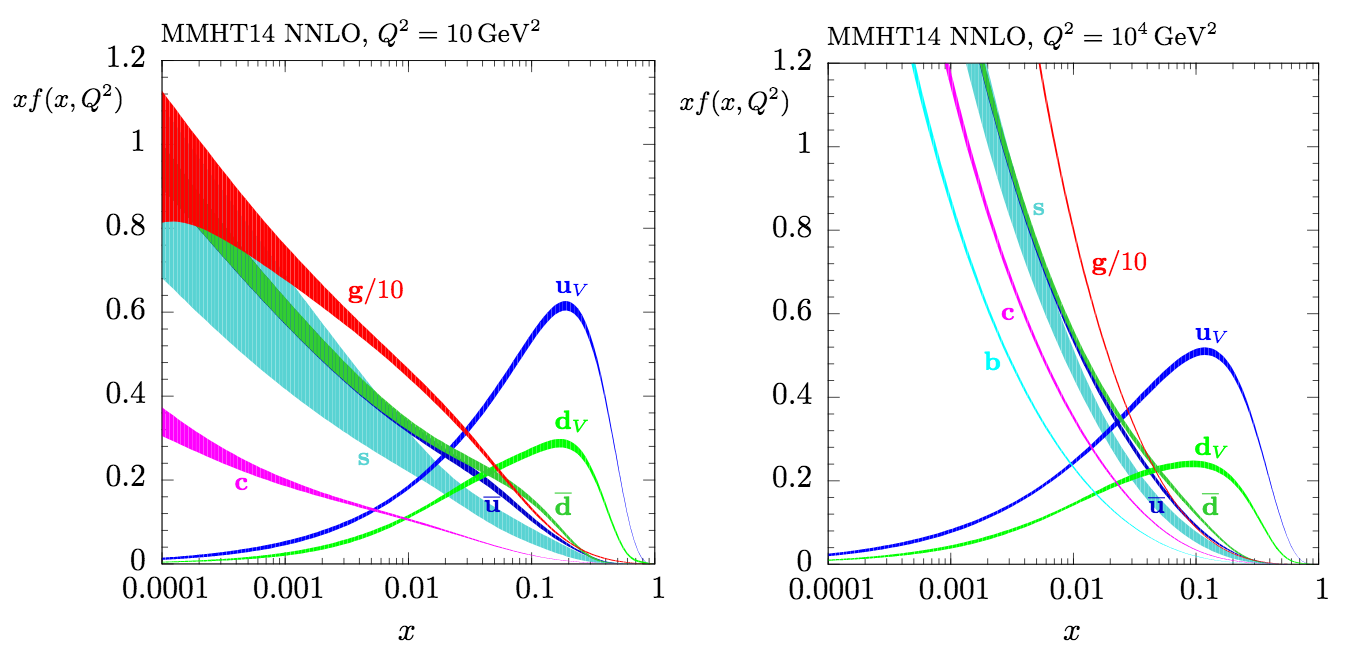
\includegraphics[width=0.9\textwidth]{figures/event_simulation/pdfs_lhc}
        \caption{
            Proton PDFs evaluated at energy scales $Q^2 = 10\,\GeV^2$ (\textit{left}) and $Q^2 = 10^4\,\GeV^2$ (\textit{right}).
            The bands indicate the 68\% confidence-level uncertainty bands.
            The valence-quark components are indicated with a subscript `v' and the sea-quark components without.
            Figures taken from Ref.~\cite{Harland-Lang:2014zoa}.
        }
        \label{fig:pdfs_lhc}
    \end{center}
\end{figure}

The remaining elements of the $pp$ event simulation described by Figure~\ref{fig:pp_sim_steps} are the parton shower (PS)
and hadronisation steps, the latter being non-perturbative and treated with phenomenological models.
The PS simulates the successive emission of quarks and gluons from the partons in the final (initial) state of the
simulated process.
In the collinear limit, the $n+1$-parton (post-emission) cross-section is related to the $n$-parton (pre-emission) crosss-section
as:
\begin{align}
    \mathrm{d}\sigma_{n+1} \approx \mathrm{d}\sigma_n \mathrm{d}P_i(z, q^2) \approx \mathrm{d}\sigma_n \frac{\alpha_s}{2\pi} \frac{\mathrm{d}q^2}{q^2} \mathrm{d}z P_{ji}(z),
    \label{eq:np1_parton_split}
\end{align}
where $\mathrm{d}P_i(z,q^2)$ is the probability that parton $i$ will split into two partons at scale $q^2$, with the parton $j$ carrying the
fraction $z$ of the momentum of the initial parton $i$.
The $P_{ji}(z)$ are Altarelli-Parisi splitting functions describing the possible parton branchings: $q \rightarrow gq$, $g \rightarrow gg$, 
and/or $g \rightarrow q\bar{q}$.
%There are three possible splittings describe by the $P_i$ in QCD: $q \rightarrow gq$, $g \rightarrow gg$, and $g \rightarrow q \bar{q}$.
The PS evolution follows by repeated implmentation of Equation~\ref{eq:np1_parton_split}, leading to arbitrarily many
parton splittings and therefore potentially arbitrarily many particles in the final state.
The basic idea, then, is to evolve the partons as above until they are below a certain energy scale, $q^2 = Q_0^2$, which is the scale
below which the hadronisation process takes place.
In typical PS MC programs, the PS evolution is performed via the construction of the Sudakov form factor {\color{red}{CHECK INDICES ETC}},
\begin{align}
    \Delta_i(q_1^2, q_2^2) = \exp \left ( - \sum\limits_j \int\limits_{q_2^2}^{q_1^2} \int\limits_{z_{\text{min}}}^{z_{\text{max}}} \mathrm{d}P_i(z,q^2) \right),
    \label{eq:sudakov_form_factor}
\end{align}
which represents the probability that a parton evolves from energy scale $q_1$ to the lower scale $q_2$ \textit{without} splitting.

The PS simulation of the final-state radiation (FSR) operates by following a \textit{forward evolution} whereby partons initially at scale $Q^2$
emit radiation at the scale $q_2$ determined by sampling Equation~\ref{eq:sudakov_form_factor}. This process is repeated and if,
for any of the partons in the final state, the $q_2^2$ value is below $Q_0^2 \approx 1\,\GeV^2$, the shower development is terminated
and hadronisation takes place {\color{red}{ISR IS THEREFORE SENSITIVE TO THE FACTORISATION SCALE AND PDF}}.
For the simulation of initial-state radiation (ISR), a \textit{backward evolution} occurs wherein the radiation is emitted
by the initiating partons. In this case the final low-energy scale is that of the ancestor partons fragmenting from the PDFs, gaining energy to take part
in the hard-scatter, and the initial energy scale is the high-energy scale of the hard-scatter.

As the partons reach the hadronisation scale, the confining nature of QCD takes over and the non-perturbative regime of QCD is reached
once again.
At this stage, the color-neutral hadrons that are observable within the detector take form.
This formation process is described by phenomenological models that capture the general
features of QCD.
The main hadronisation models used in the MC simulation relevant to the current analysis are the
Lund string model~\cite{Andersson:1983ia} and cluster hadronisation model~\cite{Webber:1983if}.
Unstable particles produced as a result of the hadronisation process are also decayed at this point;
in some cases relying on the use of dedicated programs such as \texttt{EvtGen} in the case of $b$-hadron decays~\cite{Lange:2001uf}.

\section{Monte-Carlo Event Generators}
\label{sec:mc_event_gen}

\section{Simulation of the Detector Response}
\label{sec:detector_sim}
